\documentclass[a4paper,14pt]{article}

% --- Настройка шрифтов и локализации для XeLaTeX ---
\usepackage{fontspec}
\usepackage{xunicode}
\usepackage{xltxtra}
\usepackage{polyglossia}
\setmainlanguage{russian}
\setotherlanguage{english}
\defaultfontfeatures{Ligatures=TeX}
\setmainfont{Times New Roman}
\newfontfamily\cyrillicfont{Times New Roman}
\setmonofont{Courier New}
\newfontfamily\cyrillicfonttt{Courier New}

% --- Параметры страницы по ГОСТ (Памятка: левое 3 см, правое 1 см, верхнее и нижнее по 2 см) ---
\usepackage[left=30mm, right=10mm, top=20mm, bottom=20mm]{geometry}

% --- Интервалы и абзацный отступ (1.25 см, 1.5 интервал) ---
\usepackage{indentfirst}
\setlength{\parindent}{1.25cm}
\usepackage{setspace}
\onehalfspacing

% --- Пакеты для таблиц, списков и графики ---
\usepackage{tabularx}
\usepackage{booktabs}
\usepackage{array}
\usepackage{enumitem}
\setlist{nosep, leftmargin=\parindent}
\usepackage{graphicx}
\usepackage{tikz}
\usetikzlibrary{shapes.geometric, arrows, positioning}

% --- Листинги SQL с корректным отображением пробелов в кириллице ---
\usepackage{listings}
\usepackage{xcolor}

\lstset{
    basicstyle=\ttfamily\footnotesize,
    columns=flexible,             % КЛЮЧЕВОЙ ПАРАМЕТР: отменяет схлопывание пробелов в XeLaTeX
    keepspaces=true,              % сохраняет исходные пробелы между словами
    breaklines=true,
    frame=single,
    tabsize=2,
    showstringspaces=false,
    keywordstyle=\bfseries\color{blue!70!black},
    commentstyle=\itshape\color{green!50!black},
    stringstyle=\color{red!60!black},
    numbers=none
}

% --- Оформление заголовков по стандарту ---
\usepackage{titlesec}
% Разделы: с абзацного отступа, полужирным, ПРОПИСНЫМИ буквами, без точки в конце
\titleformat{\section}[block]
  {\normalfont\bfseries\filright}
  {\hspace{1.25cm}\thesection\quad}
  {0pt}
  {\MakeUppercase}

% Подразделы: с абзацного отступа, полужирным, обычным регистром, без точки в конце
\titleformat{\subsection}[block]
  {\normalfont\bfseries\filright}
  {\hspace{1.25cm}\thesubsection\quad}
  {0pt}
  {}

\titlespacing*{\section}{0pt}{18pt}{12pt}
\titlespacing*{\subsection}{0pt}{12pt}{6pt}

% Настройка подписей к рисункам и таблицам
\usepackage[tableposition=top,figureposition=bottom]{caption}
\DeclareCaptionLabelSeparator{emdash}{~---~}
\captionsetup[figure]{
  name={Рисунок},
  labelsep=emdash,
  font={small},
  justification=centering,
  singlelinecheck=true
}
\captionsetup[table]{
  name={Таблица},
  labelsep=emdash,
  font={small},
  justification=raggedright,
  singlelinecheck=false
}

% --- Отточие в содержании ---
\usepackage{tocloft}
\renewcommand{\cftsecleader}{\cftdotfill{\cftdotsep}}
\renewcommand{\cfttoctitlefont}{\hfill\bfseries\MakeUppercase}
\renewcommand{\cftaftertoctitle}{\hfill}

\begin{document}

% =========================================================================
% ТИТУЛЬНЫЙ ЛИСТ (Стр. 1, номер не печатается)
% =========================================================================
\begin{titlepage}
    \centering
    {\small МИНИСТЕРСТВО НАУКИ И ВЫСШЕГО ОБРАЗОВАНИЯ РОССИЙСКОЙ ФЕДЕРАЦИИ}\\
    {\scriptsize \textbf{ФЕДЕРАЛЬНОЕ ГОСУДАРСТВЕННОЕ АВТОНОМНОЕ ОБРАЗОВАТЕЛЬНОЕ УЧРЕЖДЕНИЕ ВЫСШЕГО ОБРАЗОВАНИЯ}}\\
    {\bfseries «НАЦИОНАЛЬНЫЙ ИССЛЕДОВАТЕЛЬСКИЙ УНИВЕРСИТЕТ ИТМО»}\\[0.8cm]

    \textbf{Факультет безопасности информационных технологий}\\[0.6cm]

    \textbf{Направление подготовки: 10.03.01 Информационная безопасность} \\
    \textbf{Образовательная программа: «Технологии защиты информации»} \\[0.6cm]

    \textbf{Дисциплина:} \\
    \textit{\textbf{«Информационная безопасность баз данных»}} \\ [1.5cm]



    {\bfseries ОТЧЕТ ПО ЛАБОРАТОРНОЙ РАБОТЕ №1}\\
    \textit{{\bfseries «Инфологическое моделирование баз данных по методу «сущность-связь»»}}\\[4cm]

    \begin{flushright}
        \textbf{Выполнил студент(ы):} \\ [0.5em]
        группа.поток ИББД 1.7 \\ [0.5em]
        Пахомов Владимир Юрьевич / \raisebox{-0.3\height}{
\includegraphics[width=1.3cm]{sign1.png}} \\
        {\scriptsize{\textit{ФИО \hspace{2cm} Подпись \hspace{0.3cm}}}} \\ [0.3cm]
        Сивков Иван Александрович / \raisebox{-0.4\height}{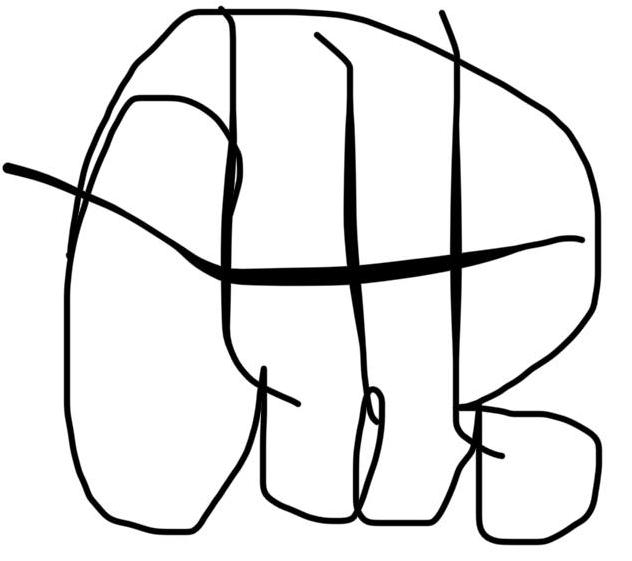
\includegraphics[width=1.1cm]{sign2.jpg}} \\
        {\scriptsize{\textit{ФИО \hspace{2cm} Подпись \hspace{0.3cm}}}} \\ [0.3cm]
        Булин Михаил Михайлович / \raisebox{-0.4\height}{
\includegraphics[width=1.3cm]{sign3.png}} \\
        {\scriptsize{\textit{ФИО \hspace{2cm} Подпись \hspace{0.3cm}}}} \\ [0.3cm]


        \textbf{Проверил:}\\ [0.5em]
        Ярцева Наталия Андреевна / \underline{\hspace{1.5cm}} \\
        {\scriptsize{\textit{ФИО \hspace{2cm} Подпись \hspace{1cm}}}} \\ [1.5cm]

        {\scriptsize \underline{\hspace{4cm}}} \\
        {\scriptsize \textit{Отметка о выполнении (один из вариантов: \\ отлично, хорошо, удовлетворительно, зачтено)}} \\
        {\scriptsize \underline{\hspace{4cm}}} \\
        {\scriptsize \textit{Дата \hspace{1.5cm}}}
    \end{flushright}

    \vfill
    Санкт-Петербург\\
    2026
\end{titlepage}

% =========================================================================
% СОДЕРЖАНИЕ (Стр. 2)
% =========================================================================
\newpage
\pagestyle{plain}
\setcounter{page}{2}

\begin{center}
    {\bfseries \MakeUppercase{Содержание}}
\end{center}
\vspace{-0.5cm}
\tableofcontents

% =========================================================================
% ВВЕДЕНИЕ
% =========================================================================
\newpage
\begin{center}
    {\bfseries \MakeUppercase{Введение}}
\end{center}
\addcontentsline{toc}{section}{ВВЕДЕНИЕ}

\textbf{Цель работы}: изучение способов семантического представления баз данных (БД), получение навыков инфологического проектирования с использованием нотации «сущность-связь».

В качестве предметной области выбрана «Информационная система морских контейнерных перевозок». Данная отрасль характеризуется распределенностью логистических цепочек, необходимостью строгого контроля за перемещением судоходных партий, учета весогабаритных характеристик контейнеров, оформления таможенной и финансовой документации, а также взаимодействием множества контрагентов с различными правами доступа к данным.

% =========================================================================
% 1. СИСТЕМНЫЙ АНАЛИЗ ИНФОРМАЦИОННОЙ СИСТЕМЫ
% =========================================================================
\newpage
\section{Системный анализ информационной системы}

\subsection{Назначение ИС и автоматизируемые процессы}
Разрабатываемая база данных предназначена для комплексного информационного обеспечения процессов морских контейнерных перевозок. База данных решает задачи централизованного учета судов, формирования графиков рейсов, регистрации заказов грузоотправителей, распределения контейнерного парка и выставления платежных документов.

В рамках ИС автоматизируются следующие основные бизнес-процессы:
\begin{itemize}
    \item регистрация клиентов и их реквизитов;
    \item оформление договоров и заявок на перевозку грузов с фиксацией весогабаритных характеристик;
    \item формирование партий грузов;
    \item планирование морских рейсов судов между портами;
    \item диспетчеризация погрузочно-разгрузочных работ и распределение заказов по рейсам;
    \item финансовый контроль, включая генерацию инвойсов и мониторинг оплаты.
\end{itemize}

\subsection{Источники данных и частота обновления}
Источниками поступления сведений в проектируемую базу данных выступают:
\begin{itemize}
    \item \textbf{Личный кабинет клиента:} электронные формы заявок на перевозку груза, реквизиты юридических лиц (поступают по мере оформления заказов, транзакционный режим обновления);
    \item \textbf{Администрация морских портов и капитании судов:} сведения о технических характеристиках причалов, осадках, прибытии и убытии судов (обновление каждые 4--6 часов или по факту швартовки);
    \item \textbf{Служба терминального контроля:} акты взвешивания контейнеров, номера защитных пломб, протоколы досмотра (поступают непрерывно в процессе обработки грузового фронта);
    \item \textbf{Бухгалтерская и биллинговая подсистема:} реестры платежей, статусы банковских транзакций (пакетное обновление 1 раз в сутки либо в режиме онлайн через банковский шлюз).
\end{itemize}

\subsection{Потребители информации и форматы представления}
Для обеспечения принципов ролевого доступа к информации в системе выделены два ключевых класса внешних потребителей данных (не считая системного администратора БД):

\textbf{1. Класс «Клиент / Грузоотправитель».} Данная категория пользователей заинтересована в отслеживании статуса своих отправлений, счетов и сохранности груза. Формат предоставления данных:
\begin{itemize}
    \item персональный электронный кабинет с таблицей заказов и инвойсов;
    \item отслеживание местоположения партии груза (наименование судна, порт отправления и назначения, расчетное время прибытия);
    \item электронная квитанция с номерами установленных запорно-пломбировочных устройств.
\end{itemize}

\textbf{2. Класс «Диспетчер флота / Логист терминала».} Данный персонал осуществляет оперативное управление движением судов и распределением контейнерной вместимости. Формат представления данных:
\begin{itemize}
    \item сводные судовые манифесты со списком принятых к перевозке контейнеров;
    \item технологические карты рейсов судов с фиксацией портов захода и допустимой осадки;
    \item контрольные ведомости распределения весовых нагрузок по контейнерам.
\end{itemize}

\subsection{Ограничения предметной области на сущности и связи}
На реляционную модель накладываются следующие жесткие бизнес-правила и ограничения целостности:
\begin{enumerate}
    \item В один и тот же рейс судно может выйти из порта отправления только один раз в заданную временную метку (не допускается пересечение рейсов одного судна во времени).
    \item Вес загруженного контейнера не может превышать сумму массы его тары и максимальной грузоподъемности.
    \item Заказ не может быть погружен на судно, рейс которого уже находится в статусе «Завершен» (\textit{Completed}) или «Отменен» (\textit{Cancelled}).
    \item Порт отправления рейса не может совпадать с портом назначения рейса.
    \item К одному заказу может быть привязан только один итоговый инвойс на оплату.
\end{enumerate}

% =========================================================================
% 2. ВЫДЕЛЕНИЕ СУЩНОСТЕЙ И ПОСТРОЕНИЕ ER-ДИАГРАММЫ
% =========================================================================
\newpage
\section{Выделение сущностей и построение ER-диаграммы}

\subsection{Описание сущностей предметной области}
В соответствии с требованиями к составу схемы выделим 7 базовых независимых сущностей (каждая содержит не менее 3 значащих атрибутов):

1. \textbf{«Клиент» (\textit{clients})}~--- отражает клиента, заключающего договор на транспортные услуги. Экземпляр: конкретная фирма или физлицо. Атрибуты: идентификатор (\textit{id}), наименование компании / ФИО (\textit{name}), адрес электронной почты (\textit{email}), контактный телефон (\textit{phone}), юридический адрес (\textit{address}).

2. \textbf{«Порт» (\textit{ports})}~--- моделирует терминальный пункт обработки судов. Экземпляр: портовый терминал. Атрибуты: идентификатор (\textit{id}), наименование порта (\textit{name}), страна расположения (\textit{country}), число причалов (\textit{dock\_count}), максимальная допустимая осадка судна (\textit{max\_draft}).

3. \textbf{«Судно» (\textit{ships})}~--- транспортная единица морского флота. Экземпляр: контейнеровоз. Атрибуты: идентификатор (\textit{id}), название судна (\textit{name}), международный номер IMO (\textit{imo\_number}), дедвейт / грузоподъемность в тоннах (\textit{deadweight}), год постройки (\textit{year\_built}).

4. \textbf{«Контейнер» (\textit{containers})}~--- унифицированная тара для перевозки. Экземпляр: стандартный контейнер. Атрибуты: идентификатор (\textit{id}), серийный номер контейнера (\textit{container\_number}), типоразмер (\textit{type}: 20FT, 40FT, Reefer), масса тары в кг (\textit{empty\_weight}), полезная вместимость в куб.м (\textit{capacity\_volume}).

5. \textbf{«Заказ» (\textit{orders})}~--- заявка на перемещение партии груза. Экземпляр: оформленное транспортное поручение. Атрибуты: идентификатор (\textit{id}), внешний ключ клиента (\textit{client\_id}), наименование груза (\textit{cargo\_name}), общий вес (\textit{cargo\_weight}), общий объем (\textit{cargo\_volume}), согласованная стоимость перевозки (\textit{total\_price}), дата оформления (\textit{created\_at}).

6. \textbf{«Рейс» (\textit{voyages})}~--- морской переход судна между портами. Экземпляр: запланированное плавание. Атрибуты: идентификатор (\textit{id}), ссылка на судно (\textit{ship\_id}), порт отправления (\textit{departure\_port\_id}), порт назначения (\textit{destination\_port\_id}), дата отхода (\textit{departure\_date}), дата прибытия (\textit{arrival\_date}), текущий статус рейса (\textit{status}).

7. \textbf{«Счет» (\textit{invoices})}~--- финансово-расчетный документ. Экземпляр: платежное требование к заказу. Атрибуты: идентификатор (\textit{id}), ссылка на заказ (\textit{order\_id}), уникальный номер счета (\textit{invoice\_number}), сумма платежа (\textit{amount}), статус оплаты (\textit{payment\_status}), дата выставления (\textit{issue\_date}).

Дополнительно для реализации связей вида «многие-ко-многим» (M:N) формируются два связующих отношения:
\begin{itemize}
    \item \textbf{«Контейнеры заказа» (\textit{order\_containers})}~--- фиксирует распределение заказа по физическим контейнерам, опломбирование и фактический вес брутто;
    \item \textbf{«Заказы рейса» (\textit{voyage\_orders})}~--- отражает судовой манифест погрузки заказов на конкретный рейс.
\end{itemize}

\subsection{Анализ связей между сущностями и классы принадлежности}
Проведем семантический анализ взаимосвязей между сущностями:

1. \textbf{Связь «Оформляет» между «Клиент» и «Заказ» (тип 1:М):}
Один клиент может оформить множество заказов. Каждый заказ обязательно оформляется ровно одним клиентом. Класс принадлежности со стороны «Заказ»~--- обязательный (заказ не существует без заказчика), со стороны «Клиент»~--- необязательный (клиент может быть только зарегистрирован и еще не совершить заказ).

2. \textbf{Связь «Выставляется по» между «Заказ» и «Счет» (тип 1:1):}
Каждому заказу соответствует один счет на оплату. Класс принадлежности со стороны «Счет»~--- обязательный (счет формируется строго под заказ), со стороны «Заказ»~--- необязательный (в момент формирования заявки счет может быть еще не сгенерирован).

3. \textbf{Связь «Включает контейнеры» между «Заказ» и «Контейнер» (тип M:N):}
Один заказ может занимать несколько контейнеров. В свою очередь, в сборных перевозках или при переиспользовании тары контейнер может участвовать в разных заказах. Реализуется через связующую сущность \textit{order\_containers}. Класс принадлежности со стороны «Заказ»~--- обязательный; со стороны «Контейнер»~--- необязательный (контейнер может стоять порожним на складе).

4. \textbf{Связь «Выполняет» между «Судно» и «Рейс» (тип 1:М):}
Одно судно совершает множество рейсов. Рейс привязан ровно к одному судну. Класс со стороны «Рейс»~--- обязательный, со стороны «Судно»~--- необязательный (новое судно может проходить докование и не иметь рейсов).

5. \textbf{Связи «Отправляется из» и «Прибывает в» между «Порт» и «Рейс» (тип 1:М):}
Каждый рейс строго определяет порт отправления и порт назначения. Класс принадлежности со стороны «Рейс»~--- обязательный, со стороны «Порт»~--- необязательный.

6. \textbf{Связь «Перевозится в рейсе» между «Рейс» и «Заказ» (тип M:N):}
В рейсе перевозится множество заказов, а составной заказ может следовать через разные рейсы. Реализуется связующей таблицей \textit{voyage\_orders}. Классы принадлежности необязательные с обеих сторон.

Сводная информация представлена в таблице \ref{tab:relations}.

\begin{table}[h!]
    \caption{Матрица связей концептуальной ER-модели}
    \label{tab:relations}
    \small
    \begin{tabularx}{\textwidth}{|X|X|c|c|c|}
        \hline
        \textbf{Сущность 1}       & \textbf{Сущность 2}             & \textbf{Тип} & \textbf{Класс Сущности 1} & \textbf{Класс Сущности 2} \\ \hline
        Клиент (\textit{clients}) & Заказ (\textit{orders})         & 1:M          & Необязательный            & Обязательный              \\ \hline
        Заказ (\textit{orders})   & Счет (\textit{invoices})        & 1:1          & Необязательный            & Обязательный              \\ \hline
        Заказ (\textit{orders})   & Контейнер (\textit{containers}) & M:N          & Обязательный              & Необязательный            \\ \hline
        Судно (\textit{ships})    & Рейс (\textit{voyages})         & 1:M          & Необязательный            & Обязательный              \\ \hline
        Порт (\textit{ports})     & Рейс (\textit{voyages})         & 1:M          & Необязательный            & Обязательный              \\ \hline
        Рейс (\textit{voyages})   & Заказ (\textit{orders})         & M:N          & Необязательный            & Необязательный            \\ \hline
    \end{tabularx}
\end{table}

\subsection{Графическое представление ER-диаграммы}
Концептуальная схема связей предметной области представлена на рисунке \ref{fig:er_diagram}.

\begin{figure}[h!]
    \centering
    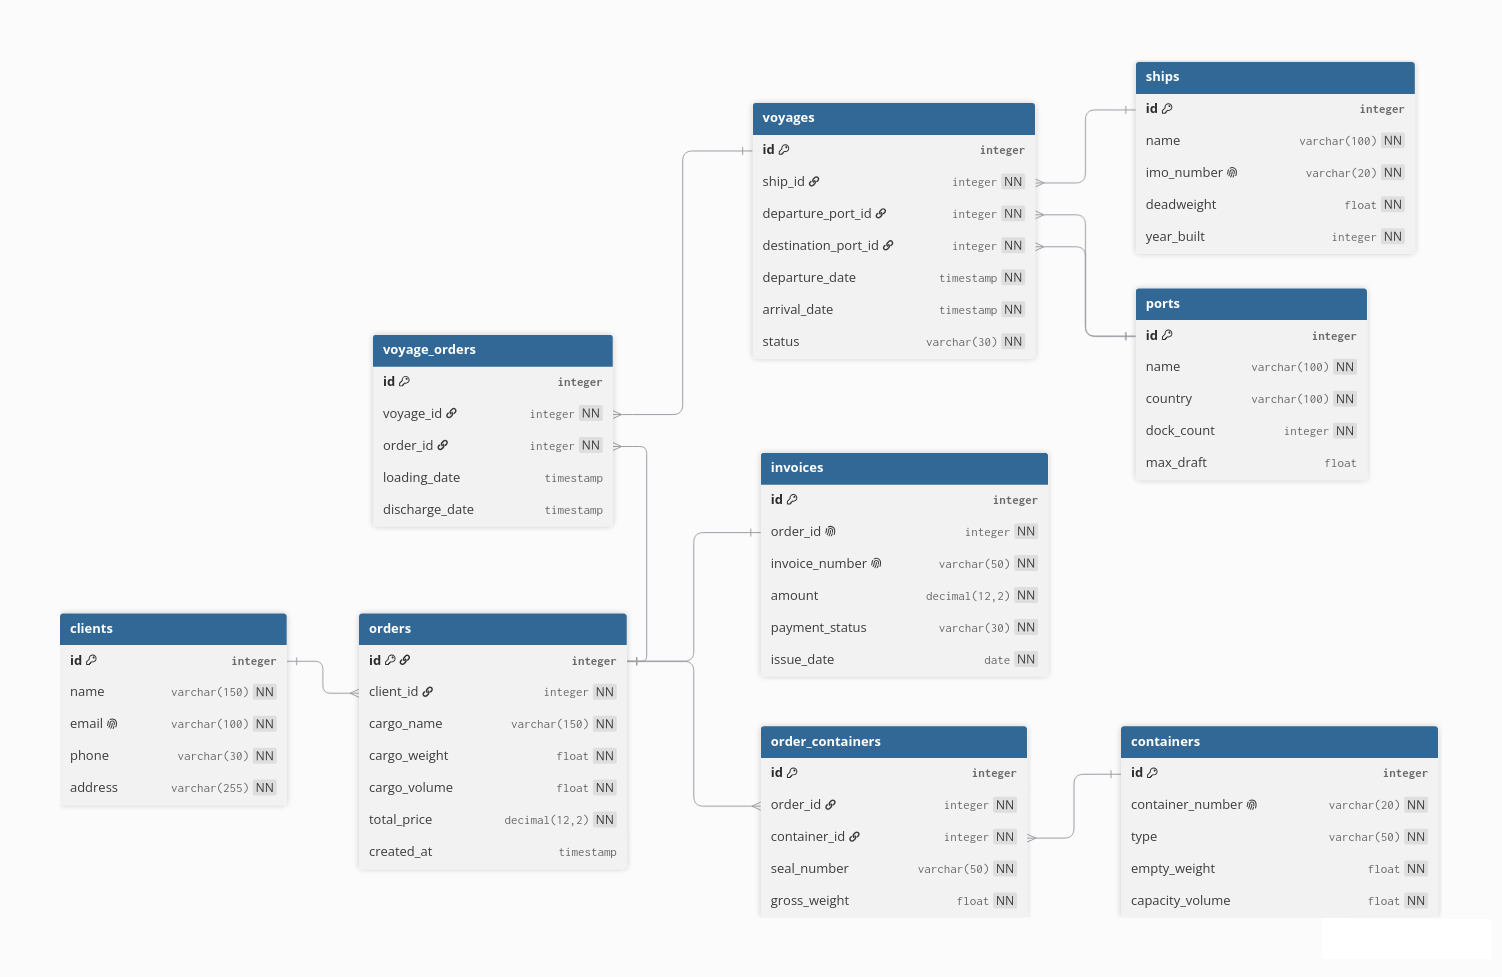
\includegraphics[width=1.02\textwidth]{ER_diagram.png}
    \caption{Концептуальная ER-диаграмма предметной области}
    \label{fig:er_diagram}
\end{figure}

% =========================================================================
% 3. ПРЕОБРАЗОВАНИЕ ER-ДИАГРАММЫ В СХЕМУ ОТНОШЕНИЙ
% =========================================================================
\newpage
\section{Преобразование ER-диаграммы в схему отношений}

Преобразование концептуальной модели в логическую схему реляционной базы данных выполняется на основе формализованных правил:

1. \textbf{Преобразование связи 1:M с обязательным классом подчиненной сущности:}
Связь «Оформляет» между «Клиент» и «Заказ». Первичный ключ сущности со стороны «1» (\textit{clients.id}) переносится в качестве внешнего ключа (Foreign Key, FK) в отношение со стороны «M» (\textit{orders.client\_id}) с ограничением \textit{NOT NULL}.
Аналогично преобразуются связи судна с рейсом (\textit{voyages.ship\_id}) и портов захода (\textit{voyages.departure\_port\_id}, \textit{voyages.destination\_port\_id}).

2. \textbf{Преобразование связи 1:1:}
Связь между сущностями «Заказ» и «Счет». Первичный ключ отношения «Заказ» (\textit{orders.id}) включается в отношение «Счет» (\textit{invoices.order\_id}) с наложением уникального индекса (\textit{UNIQUE}) и запрета на нулевые значения (\textit{NOT NULL}), что обеспечивает строгое сохранение кардинальности 1:1.

3. \textbf{Преобразование связей M:N:}
Связи «Заказ --- Контейнер» и «Рейс --- Заказ» преобразуются в отдельные связующие таблицы (\textit{order\_containers} и \textit{voyage\_orders}). В каждую из них включаются первичные ключи ассоциированных сущностей в роли внешних ключей, а также собственные атрибуты взаимосвязи (контрольная масса, метки времени погрузки и выгрузки).

Итоговый перечень полученных предварительных отношений:
\begin{enumerate}
    \item $R_1$~--- \textbf{clients} (\underline{id}, name, email, phone, address);
    \item $R_2$~--- \textbf{ports} (\underline{id}, name, country, dock\_count, max\_draft);
    \item $R_3$~--- \textbf{ships} (\underline{id}, name, imo\_number, deadweight, year\_built);
    \item $R_4$~--- \textbf{containers} (\underline{id}, container\_number, type, empty\_weight, capacity\_volume);
    \item $R_5$~--- \textbf{orders} (\underline{id}, cargo\_name, cargo\_weight, cargo\_volume, total\_price, created\_at, \textit{client\_id});
    \item $R_6$~--- \textbf{voyages} (\underline{id}, departure\_date, arrival\_date, status, \textit{ship\_id}, \textit{departure\_port\_id}, \textit{destination\_port\_id});
    \item $R_7$~--- \textbf{invoices} (\underline{id}, invoice\_number, amount, payment\_status, issue\_date, \textit{order\_id});
    \item $R_8$~--- \textbf{order\_containers} (\underline{id}, seal\_number, gross\_weight, \textit{order\_id}, \textit{container\_id});
    \item $R_9$~--- \textbf{voyage\_orders} (\underline{id}, loading\_date, discharge\_date, \textit{voyage\_id}, \textit{order\_id}).
\end{enumerate}

% =========================================================================
% 4. ПРИВЕДЕНИЕ ОТНОШЕНИЙ БД К 3НФ
% =========================================================================
\newpage
\section{Приведение отношений БД к третьей нормальной форме}

Для доказательства корректности полученной схемы выполним проверку соблюдения требований нормализации:

\subsection{Проверка требований Первой нормальной формы (1НФ)}
Отношение находится в 1НФ, если все используемые домены содержат только неделимые скалярные значения, и в отношении отсутствуют повторяющиеся группы или массивы.
\begin{itemize}
    \item В атрибутах \textit{clients.phone}, \textit{clients.email} хранятся единичные строковые литералы. Разделение ФИО и адресов на более мелкие поля не требуется для целей решаемых аналитических задач.
    \item Связи «многие-ко-многим» вынесены в таблицы $R_8$ и $R_9$, что исключило списки идентификаторов контейнеров в строках таблицы \textit{orders}.
\end{itemize}
Следовательно, все отношения $R_1$--$R_9$ находятся в 1НФ.

\subsection{Проверка требований Второй нормальной формы (2НФ)}
Отношение находится во 2НФ, если оно находится в 1НФ и каждый неключевой атрибут функционально полно зависит от первичного ключа (отсутствуют частичные функциональные зависимости от части составного ключа).
\begin{itemize}
    \item Во всех таблицах первичные ключи являются простыми суррогатными ключами (\textit{id}).
    \item Ни в одной таблице не используется составной первичный ключ, поэтому возникновение частичной функциональной зависимости теоретически невозможно.
\end{itemize}
Следовательно, все отношения находятся во 2НФ.

\subsection{Проверка требований Третьей нормальной формы (3НФ)}
Отношение находится в 3НФ, если оно находится во 2НФ и отсутствуют транзитивные функциональные зависимости неключевых атрибутов от первичного ключа.
\begin{itemize}
    \item В таблице \textit{orders} не хранятся реквизиты клиента (название, телефон); они извлекаются через ключ \textit{client\_id}.
    \item В таблице \textit{voyages} не дублируются наименования портов и параметры судна; присутствуют исключительно прямые ссылки \textit{ship\_id} и \textit{port\_id}.
    \item В таблице \textit{order\_containers} масса тары контейнера не хранится повторно, фиксируется исключительно измеренный фактический вес конкретной погрузки (\textit{gross\_weight}).
\end{itemize}

% =========================================================================
% 5. МОДЕЛИРОВАНИЕ УРОВНЯ ПРЕДСТАВЛЕНИЙ (VIEW)
% =========================================================================
\newpage
\section{Моделирование уровня представлений информационной системы}

Для каждого из двух выделенных классов внешних потребителей разработано по 2 специализированных представления (\textit{VIEW}). Каждое представление объединяет атрибуты из двух и более связанных отношений.

\subsection{Представления для потребителя «Клиент / Грузоотправитель»}

\textbf{1. Представление \texttt{view\_client\_orders} («Реестр заказов и оплат»).}
Обеспечивает вывод информации о статусе обработки заказа, присвоенных пломбах и выставленном финансовом счете. Использует объединение таблиц \textit{orders}, \textit{invoices} и \textit{order\_containers}.

\begin{lstlisting}[language=SQL]
CREATE VIEW view_client_orders AS
SELECT 
    o.id AS order_id,
    o.client_id,
    o.cargo_name,
    o.total_price,
    i.invoice_number,
    i.payment_status,
    COUNT(oc.container_id) AS containers_count,
    SUM(oc.gross_weight) AS actual_gross_weight
FROM orders o
LEFT JOIN invoices i ON o.id = i.order_id
LEFT JOIN order_containers oc ON o.id = oc.order_id
GROUP BY o.id, o.client_id, o.cargo_name, o.total_price, 
         i.invoice_number, i.payment_status;
\end{lstlisting}

\textbf{2. Представление \texttt{view\_client\_tracking} («Маршрутный трекинг груза»).}
Предоставляет клиенту сведения о рейсе, судне и плановых датах доставки. Затрагивает таблицы \textit{orders}, \textit{voyage\_orders}, \textit{voyages}, \textit{ships}, \textit{ports}.

\begin{lstlisting}[language=SQL]
CREATE VIEW view_client_tracking AS
SELECT 
    o.id AS order_id,
    o.client_id,
    o.cargo_name,
    s.name AS vessel_name,
    p_dep.name AS port_of_loading,
    p_arr.name AS port_of_discharge,
    v.departure_date,
    v.arrival_date,
    v.status AS voyage_status
FROM orders o
JOIN voyage_orders vo ON o.id = vo.order_id
JOIN voyages v ON vo.voyage_id = v.id
JOIN ships s ON v.ship_id = s.id
JOIN ports p_dep ON v.departure_port_id = p_dep.id
JOIN ports p_arr ON v.destination_port_id = p_arr.id;
\end{lstlisting}

\subsection{Представления для потребителя «Диспетчер флота / Логист терминала»}

\textbf{1. Представление \texttt{view\_voyage\_manifest} («Судовой грузовой манифест»).}
Позволяет диспетчеру оценить коммерческую загрузку конкретного рейса, суммарную массу принятого груза и соответствие дедвейту судна. Задействует отношения \textit{voyages}, \textit{ships}, \textit{ports}, \textit{voyage\_orders}, \textit{orders}.

\begin{lstlisting}[language=SQL]
CREATE VIEW view_voyage_manifest AS
SELECT 
    v.id AS voyage_id,
    s.name AS ship_name,
    s.deadweight AS ship_capacity_tons,
    p1.name AS origin_port,
    p2.name AS destination_port,
    COUNT(vo.order_id) AS total_orders_assigned,
    COALESCE(SUM(o.cargo_weight), 0) / 1000.0 AS total_cargo_tons
FROM voyages v
JOIN ships s ON v.ship_id = s.id
JOIN ports p1 ON v.departure_port_id = p1.id
JOIN ports p2 ON v.destination_port_id = p2.id
LEFT JOIN voyage_orders vo ON v.id = vo.voyage_id
LEFT JOIN orders o ON vo.order_id = o.id
GROUP BY v.id, s.name, s.deadweight, p1.name, p2.name;
\end{lstlisting}

\textbf{2. Представление \texttt{view\_container\_safety\_audit} («Ведомость контроля веса и пломб»).}
Служит для проверки безопасности погрузки, выявления перегруженных контейнеров и контроля целостности ЗПУ. Использует объединение таблиц \textit{order\_containers}, \textit{containers}, \textit{orders}, \textit{clients}.

\begin{lstlisting}[language=SQL]
CREATE VIEW view_container_safety_audit AS
SELECT 
    c.container_number,
    c.type AS container_type,
    c.empty_weight AS tare_weight,
    oc.seal_number,
    oc.gross_weight,
    (oc.gross_weight - c.empty_weight) AS net_cargo_weight,
    o.id AS order_id,
    cl.name AS shipper_name
FROM order_containers oc
JOIN containers c ON oc.container_id = c.id
JOIN orders o ON oc.order_id = o.id
JOIN clients cl ON o.client_id = cl.id;
\end{lstlisting}

% =========================================================================
% ЗАКЛЮЧЕНИЕ
% =========================================================================
\newpage
\begin{center}
    {\bfseries \MakeUppercase{Заключение}}
\end{center}
\addcontentsline{toc}{section}{ЗАКЛЮЧЕНИЕ}

В ходе выполнения лабораторной работы была успешно спроектирована инфологическая и реляционная модель базы данных «Информационная система контейнерных перевозок».

В рамках работы были достигнуты следующие результаты:
\begin{enumerate}
    \item Выполнен системный анализ предметной области логистики морских перевозок, сформулированы ключевые цели автоматизации и ограничения целостности данных.
    \item Выделено 7 фундаментальных отношений схемы, каждое из которых содержит не менее трех атрибутов, а также 2 промежуточные таблицы для реализации связей вида M:N.
    \item Проведен анализ кардинальности и классов принадлежности связей, после чего по формальным правилам осуществлен переход от концептуальной ER-модели к логической схеме базы данных.
    \item Обосновано нахождение всех полученных отношений в третьей нормальной форме (3НФ), что исключает избыточность информации и риски аномалий модификации.
    \item Спроектирован уровень представлений: сформировано 4 представления (\textit{VIEW}), реализующие ролевое разграничение доступа для клиентов и диспетчеров морского терминала с агрегацией данных из связанных таблиц.
\end{enumerate}

Разработанная модель данных полностью готова к практической реализации на базе современных СУБД.


\end{document}
